\documentclass[english, a4paper,12pt]{article}
\usepackage[a4paper, top=2cm, bottom=2cm,right=2cm,left=2cm]{geometry}
\date{} 
\usepackage[utf8]{vietnam}
\usepackage{textcomp, graphicx, titling, tkz-tab, changepage}
\usepackage{changepage, xcolor, amsmath, fancyvrb, minted, caption} 
\definecolor{LightGray}{gray}{0.95}

\usepackage[english]{babel}
\addto\captionsenglish{
  \renewcommand{\contentsname}
  {Table of Contents}
}

\begin{document}
\begin{titlepage}
\begin{center}
\textbf{UNIVERSITY OF INFORMATION TECHNOLOGY}

\textbf{FACULTY OF COMPUTER SCIENCE}

\vspace{1cm}

\vspace{1cm}

\textbf{REPORT UCS/A STAR SEARCH FOR SOKOBAN}

\vspace{2cm}

\includegraphics[width= 5cm]{logo.png}
\vspace{2cm}

\textbf{Instructor: } Luong Ngoc Hoang

\vspace{0.5cm}

\textbf{Student:} Ha Huy Hoang - 22520460
\vspace{0.5cm}
\\
\textbf{Class:} CS106.O21
\vspace{2cm}
\tableofcontents
\end{center}
\end{titlepage}
\subsection*{Note}
\hspace*{7mm}Level 17 has no solution (all nodes have been explored, and there is no way to solve it)and Level 18, I’ve run all the algorithms for over an hour, but there are still no results. Therefore, I won’t include Level 17 and Level 18 in the statistics table.
\section*{1. UCS}
\addcontentsline{toc}{section}{1. UCS}
\small\begin{minipage}{.35\textwidth}
\begin{tabular}{|c|c|c|c|}
\hline
Level & Steps & Time & Nodes  \\
\hline
1 & 12 & 0.16 & 818\\
2 & 9 & 0.04 & 82\\
3 & 15 & 0.29 & 677 \\
4 & 7 & 0.03 & 89\\
5 & 20 & 236.44 & 687417 \\
6 & 19 & 0.08 & 250\\
7 & 21 & 1.21 & 7110\\
8 & 97 & 0.55 & 2425\\
9 & 8 & 0.07 & 105\\
10 & 33 & 0.07 & 230\\
11 & 34  & 0.07 & 300\\
12 & 23 & 0.53 & 1266\\
13 & 31 & 0.42 & 2382\\
14 & 23 & 5.86 & 27440\\
15 & 105 & 0.6 & 2519\\
16 & 34 & 35.33 & 70366 \\
\hline
\end{tabular}
\end{minipage}
\begin{minipage}{.7\textwidth}
The UCS (Uniform Cost Search) algorithm uses a priority queue to sort based on the cost of the path (which is the number of steps without moving boxes) using cost function.\\
\hspace*{35mm}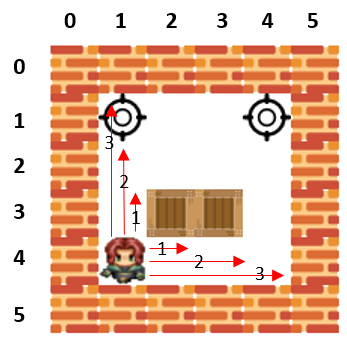
\includegraphics[width=4cm]{Level1_UCS.png}\\
\hspace*{10mm}\textbf{Image 1.} Cost Distance in begin state of Level 1
\end{minipage}
\vspace*{3mm}
\\
Mathematically:
\vspace*{3mm}\\
\hspace*{5mm}$Cost = actions.count('l') + actions.count('r') + actions.count('d') + actions.count('u')$
\vspace*{3mm}
\\
Code:
\small\begin{minted}[bgcolor=LightGray]{Python}
def cost(actions):
    return len([x for x in actions if x.islower()])
\end{minted}

\section*{2. A Star Search}
\addcontentsline{toc}{section}{2. A Star Search}
The A* search algorithm itself consists of two different heuristic functions for only one algorithm. The first one is the heuristic to calculate the cost for Sokoban in each iteration. And the other one is the heuristic to estimate the distance from the boxes to the goals.\\

The first heuristic is illustrated as the cost function of UCS:
\vspace*{5mm}\\
\hspace*{5mm}$Cost = actions.count('l') + actions.count('r') + actions.count('d') + actions.count('u')$
\\

And the second one can be use other heuristics as: \textbf{2.1.} Mahattan Distance, \textbf{2.2. } Euclidean Distance and \textbf{2.3. } Chebyshev Distance.
\newpage
\subsection*{2.1. Using Mahattan Distance}
\addcontentsline{toc}{subsection}{2.1. Using Mahattan Distance}
\small\begin{minipage}{.35\textwidth}
\begin{tabular}{|c|c|c|c|}
\hline
Level & Steps & Time(s) & Nodes \\
\hline
1 & 13 & 0.05 & 91 \\
2 & 9 & 0.03 & 39 \\
3 & 15 & 0.05 & 58 \\
4 & 7 & 0.01 & 19 \\
5 & 22 & 0.25 & 493 \\
6 & 19 & 0.07 & 214 \\
7 & 21 & 0.19 & 791 \\
8 & 97 & 0.62 & 2353 \\
9 & 8 & 0.03 & 38 \\
10 & 33 & 0.08 & 199 \\
11 & 34 & 0.08 & 285 \\
12 & 23 & 0.14 & 573 \\
13 & 31 & 0.40 & 1692 \\
14 & 23 & 1.95 & 8079 \\
15 & 105 & 0.68 & 2187 \\
16 & 42 & 0.78 & 1294 \\
\hline
\end{tabular}
\end{minipage}
\begin{minipage}{.7\textwidth}
\hspace*{5mm}Manhattan  Distance,  also  known  as  city  block distance  and  it  is  used  the  calculate  the  distance  between two points in a grid-based path. By considering only vertical and  horizontal  movements  and  no  diagonal  movement allowed.  The  name  derives  from  the  grid  layout  of  most streets in Manhattan, which forms square block.$^{(1)}$ \\
\hspace*{5mm}In this prolem, the algorithm will compute the absolute values of differences between boxes and goals.

\hspace*{35mm}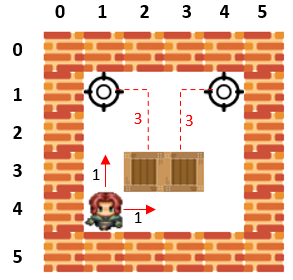
\includegraphics[width=4cm]{Level1_mah.png}\\
\hspace*{10mm}\textbf{Image 2.1.} Mahattan Distance in begin state of Level 1
\end{minipage}
\vspace*{3mm}
\\
Mathematically: \\
\hspace*{10mm}$Mahattan\_Dist = |x.Boxes - x.Goals| + |y.Boxes - y.Goals|$\\
Code:
\begin{minted}[bgcolor=LightGray]{Python}
    def mahattan_dist(posPlayer, posBox):
        distance = 0
        completes = set(posGoals) & set(posBox)
        sortposBox = list(set(posBox).difference(completes))
        sortposGoals = list(set(posGoals).difference(completes))
        for i in range(len(sortposBox)):
            distance += (abs(sortposBox[i][0] - sortposGoals[i][0])) 
                     + (abs(sortposBox[i][1] - sortposGoals[i][1]))
        return distance
\end{minted}

\subsection*{2.2. Using Euclidean Distance}
\addcontentsline{toc}{subsection}{2.2. Using Euclidean Distance}
\begin{minipage}{.35\textwidth}
\begin{tabular}{|c|c|c|c|}
\hline
Level & Steps & Time(s) & Nodes \\
\hline
1 & 13 & 0.09 & 243 \\
2 & 9 & 0.01 & 39 \\
3 & 15 & 0.04 & 48 \\
4 & 7 & 0.02 & 29 \\
5 & 22 & 0.27 & 499 \\
6 & 19 & 0.08 & 219 \\
7 & 21 & 0.39 & 1117 \\
8 & 97 & 0.80 & 2366 \\
9 & 8 & 0.02 & 37 \\
10 & 33 & 0.09 & 199 \\
11 & 34 & 0.10 & 285 \\
12 & 23 & 0.22 & 625 \\
13 & 31 & 0.49 & 1807 \\
14 & 23 & 2.58 & 9894 \\
15 & 105 & 0.71 & 2248 \\
16 & 36 & 1.18 & 1880 \\
\hline
\end{tabular}
\end{minipage}
\begin{minipage}{.7\textwidth}
\begin{adjustwidth}{1mm}{}
\hspace*{3mm}The  Euclidean  distance represents  the  shortest distance between two  points  in  a 2D or 3D space, is calculated as the ‘bird’s flight path’ - the length of the straight line connecting from the boxes to goals (closest to the box under consideration).
\end{adjustwidth}

\hspace*{35mm}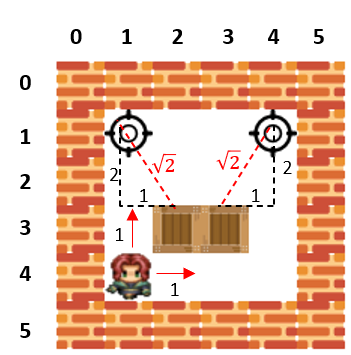
\includegraphics[width=4cm]{Level1_EUC.png}\\
\hspace*{10mm}\textbf{Image 2.2.} Euclidean Distance in begin state of Level 1
\end{minipage}
\newpage
Mathematically: 
\vspace*{3mm}\\
\hspace*{10mm}$Euclidean\_Dist = \sqrt{(x.Boxes - x.Goals)^2 + (y.Boxes - y.Goals)^2}$ \\
Code:
\begin{minted}[bgcolor=LightGray]{Python}
    def euclidean_dist(posPlayer, posBox):
        distance = 0
        completes = set(posGoals) & set(posBox)
        sortposBox = list(set(posBox).difference(completes))
        sortposGoals = list(set(posGoals).difference(completes))
        for i in range(len(sortposBox)):
            distance += math.sqrt((sortposBox[i][0] - sortposGoals[i][0])**2 
                        + (sortposBox[i][1] - sortposGoals[i][1])**2)
        return distance
\end{minted}
\subsection*{2.3. Using Chebyshev Distance}
\addcontentsline{toc}{subsection}{2.1. Using Chebyshev Distance}
\begin{minipage}{.35\textwidth}
\begin{tabular}{|c|c|c|c|}
\hline
Level & Steps & Time(s) & Nodes \\
\hline
1 & 12 & 0.09 & 261 \\
2 & 9 & 0.03 & 39 \\
3 & 15 & 0.04 & 54 \\
4 & 7 & 0.02 & 35 \\
5 & 20 & 0.17 & 386 \\
6 & 19 & 0.07 & 231 \\
7 & 21 & 0.38 & 1835 \\
8 & 97 & 0.46 & 2432 \\
9 & 8 & 0.02 & 34 \\
10 & 33 & 0.08 & 204 \\
11 & 34 & 0.07 & 288 \\
12 & 23 & 0.16 & 769 \\
13 & 31 & 0.34 & 1997 \\
14 & 23 & 3.10 & 12948 \\
15 & 105 & 0.62 & 2360 \\
16 & 34 & 0.64 & 1533 \\
\hline
\end{tabular}
\end{minipage}
\begin{minipage}{.7\textwidth}
Chebyshev distance, named  after  Pafnuty  Chebyshev, is a  metric  that defines  the  distance between  two  points in  a grid,  allowing  for  diagonal  movement.  It  is  especially relevant  in  chessboard-like  environments  where  eight possible movement directions exist (including diagonals). It essentially captures the maximum of the absolute difference in x and y coordinates.$^{(2)}$\\
\hspace*{35mm}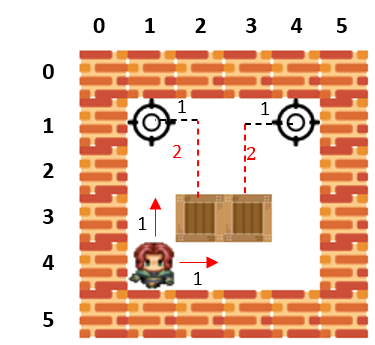
\includegraphics[width=4cm]{Level1_CHE.png}\\
\hspace*{10mm}\textbf{Image 2.3. } Chebyshev Distance in begin state of Level 1
\end{minipage}
\vspace*{3mm}
\\
Mathematically: 
\vspace*{3mm}\\
\hspace*{10mm}$Chebyshev\_Dist = max(|x.Boxes - x.Goals|, |y.Boxes - y.Goals|)$\\
Code:
\begin{minted}[bgcolor=LightGray]{Python}
    def chebyshev_dist(posPlayer, posBox):
        distance = 0
        completes = set(posGoals) & set(posBox)
        sortposBox = list(set(posBox).difference(completes))
        sortposGoals = list(set(posGoals).difference(completes))
        for i in range(len(sortposBox)):
            distance += max((abs(sortposBox[i][0] - sortposGoals[i][0])),
                        (abs(sortposBox[i][1] - sortposGoals[i][1])))
        return distance
\end{minted}
\section*{3. Comparison}
\addcontentsline{toc}{section}{3. Comparison}
\subsection*{3.1. UCS vs A Star Search}
\addcontentsline{toc}{subsection}{3.1. UCS vs A Star Search}
\begin{table}[h]
\small\begin{minipage}{0.5\textwidth}
\centering
\begin{tabular}{|c|c|c|c|c|}
\hline
Level & UCS & MAH & EUC & CHE \\
\hline
1 & 12 & 13 & 13 & 12 \\
2 & 9 & 9 & 9 & 9 \\
3 & 15 & 15 & 15 & 15 \\
4 & 7 & 7 & 7 & 7\\
5 & 20 & 22 & 22 & 20\\
6 & 19 & 19 & 19 & 19\\
7 & 21 & 21 & 21 & 21\\
8 & 97 & 97 & 97 & 97\\
9 & 8 & 8 & 8 & 8\\
10 & 33 & 33 & 33 & 33\\
11 & 34 & 34 & 34 & 34\\
12 & 23 & 23 & 23 & 23\\
13 & 31 & 31 & 31 & 31\\
14 & 23 & 23 & 23 & 23 \\
15 & 105 & 105 & 105 & 105\\
16 & 34 & 42 & 36 & 34\\
\hline
\end{tabular}
\caption*{\textbf{Image 3.1.1.} Movement step statistics}
\end{minipage}
\small\begin{minipage}{0.5\textwidth}
\centering
\small\begin{tabular}{|c|c|c|c|c|}
\hline
Level & UCS & MAH & EUC & CHE \\
\hline
1 & 0.16 & 0.05 & 0.09 & 0.09\\
2 & 0.04 & 0.03 & 0.01 & 0.03 \\
3 & 0.29 & 0.05 & 0.04 & 0.04 \\
4 & 0.03 & 0.01 & 0.02 & 0.02\\
5 & 236.44 & 0.25 & 0.27 & 0.17\\
6 & 0.08 & 0.07 & 0.08 & 0.07\\
7 & 1.21 & 0.19 & 0.39 & 0.38\\
8 & 0.55 & 0.62 & 0.80 & 0.46\\
9 & 0.07 & 0.03 & 0.02 & 0.02\\
10 & 0.07 & 0.08 & 0.09 & 0.08\\
11 & 0.07 & 0.08 & 0.10 & 0.07\\
12 & 0.53 & 0.14 & 0.22 & 0.16\\
13 & 0.42 & 0.40 & 0.49 & 0.34\\
14 & 5.86 & 1.95 & 2.58 & 3.10 \\
15 & 0.6 & 0.68 & 0.71 & 0.62\\
16 & 35.33 & 0.78 & 1.18 & 0.64\\
\hline
\end{tabular}
\caption*{\textbf{Image 3.1.2.} Time solving statistics(s)}
\end{minipage}
\end{table}
\begin{itemize}
    \item Uniform Cost Search (UCS): This algorithm has varying performance. For some cases, it finds the solution with fewer steps and less time. However, in other cases, it takes significantly more time and explores a large number of nodes, which indicates a high computational cost.
    \item A* with Manhattan Distance (MAH): This algorithm consistently finds the solution with fewer steps, less time, and fewer nodes explored compared to UCS. This suggests that A* with Manhattan distance is more efficient than UCS for these cases.
    \item A* with Euclidean Distance (EUC): Similar to A* with Manhattan distance, this algorithm also performs better than UCS in terms of steps, time, and nodes explored. However, it seems to be slightly less efficient than A* with Manhattan distance as it generally takes more time and explores more nodes.
    \item A* with Chebyshev Distance (CHE): This algorithm also outperforms UCS. It finds the solution with fewer steps and less time, and explores fewer nodes than UCS. Its performance is comparable to A* with Manhattan and Euclidean distances.
\end{itemize}

\hspace*{50mm}\begin{tabular}{|c|c|c|c|c|}
\hline
Level & UCS & MAH & EUC & CHE \\
\hline
1 & 818 & 91 & 243 & 261 \\
2 & 82 & 39 & 39 & 39\\
3 & 677 & 58 & 48 & 54 \\
4 & 89 & 19 & 29 & 35\\
5 & 687417 & 493 & 499 & 386\\
6 & 250 & 214 & 219 & 231\\
7 & 7110 & 791 & 1117 & 1835\\
8 & 2425 & 2353 & 2366 & 2432\\
9 & 105 & 38 & 37 & 34 \\
10 & 230 & 199 & 199 & 204\\
11 & 300 & 285 & 285 & 288 \\
12 & 1266 & 573 & 625 & 769 \\
13 & 2382 & 1692& 1807 & 1997 \\
14 & 27440 & 8079 & 9894 & 12948 \\
15 & 2519 & 2187 & 2248 & 2360 \\
16 & 70366 & 1294 & 1880 & 1533 \\
\hline
\end{tabular}
\vspace*{3mm}
\\
\hspace*{55mm}\textbf{Image 3.1.3. } Explored nodes statistics
\vspace*{3mm}
\\
\hspace*{7mm}In conclusion, A* with heuristic functions (Manhattan, Euclidean, or Chebyshev distance) generally performs better than UCS in terms of the number of steps, time, and nodes explored. Because Uniform Cost Search (UCS) does not use a heuristic function, it may open many nodes in the exploratory set, including those far from the goal. This leads to UCS often taking more time and traversing a larger number of nodes compared to A*. This is particularly noticeable on large maps, where A* can be much more efficient than UCS. However, on simple maps, the difference between the run times of UCS and A* may not be significant, and one could say the performance of the two algorithms is comparable. Among the A* algorithms, A* with Manhattan distance seems to be the most efficient. Nevetheless, the best choice of algorithm may depend on the specific characteristics of the problem and the computational resources available.
\subsection*{3.2. The efficient of A Star Search}
\addcontentsline{toc}{subsection}{3.2. The efficiency of A Star Search}
\small\begin{minipage}{0.4\textwidth}
\begin{tabular}{|c|c|c|c|c|}
\hline
Level & BFS & MAH & EUC & CHE \\
\hline
1 & 12 & 13 & 13 & 12 \\
2 & 9 & 9 & 9 & 9 \\
3 & 15 & 15 & 15 & 15 \\
4 & 7 & 7 & 7 & 7\\
5 & 20 & 22 & 22 & 20\\
6 & 19 & 19 & 19 & 19\\
7 & 21 & 21 & 21 & 21\\
8 & 97 & 97 & 97 & 97\\
9 & 8 & 8 & 8 & 8\\
10 & 33 & 33 & 33 & 33\\
11 & 34 & 34 & 34 & 34\\
12 & 23 & 23 & 23 & 23\\
13 & 31 & 31 & 31 & 31\\
14 & 23 & 23 & 23 & 23 \\
15 & 105 & 105 & 105 & 105\\
16 & 34 & 42 & 36 & 34\\
\hline
\end{tabular}
\end{minipage}
\begin{minipage}{0.6\textwidth}
As we can see, almost all levels have the optimal solution, except for two levels which show differences:
\begin{itemize}
    \item Level 5: BFS and CHE require 20 steps, while MAH and EUC require 22 steps.
    \item Level 16: BFS and CHE require 34 steps, MAH requires 42 steps, and EUC requires 36 steps. 
\end{itemize}
The number of steps can vary between algorithms due to the way they identify and explore the search space. In the case of A* (with MAH, EUC, and CHE heuristics), it may find a not optimal route compared to BFS (the algorithm find the shortest solution), depending on the specific characteristics of the map and the start and end positions.
\end{minipage}
\vspace*{2mm}
\\
\textbf{REFERENCES}
\vspace*{2mm}
\\
\text{[1]}, [2]. Sai Prasad Gudari, Dr. Vadivu G. (2023, November). \textit{A Study on the Performance of the A-Star Algorithm with Various Heuristics in Grids and Graphs}.
\end{document}